\documentclass[11pt]{article}
%%%%%%%%%%%%%%%%%%%%%%%%%%%%%%%%%%%%%%%%%

\usepackage{amscd}
\usepackage{amsmath}
\usepackage{amssymb}
\usepackage{amsthm}

\usepackage{float}
\usepackage{epsfig}
\usepackage{verbatim}
\usepackage{graphicx}
\usepackage{amsthm}
\usepackage{multirow}
\usepackage{hyperref}
\pagestyle{empty}
\usepackage{color}
\usepackage[left=3cm,top=2.5cm,right=3cm,bottom=3cm]{geometry} % Document margins
%\usepackage[all,dvips]{xy}


\begin{comment}  

This LaTeX document is a template to be used by Bates mathematics rising seniors to create a thesis proposal. 

As a guide, the document is already filled out to represent a fictitious proposal, and all you need to do is modify the entries below to represent your own proposal.

A PDF version of the fictitious proposal is available on the department's FAQ and Policies pages, at
http://abacus.bates.edu/acad/depts/math/faq.html
and
http://abacus.bates.edu/acad/depts/math/policies.html
respectively.

Once you have finished your proposal, export it to a PDF file. Give the file a USEFUL name, for example, RiemannThesisProposal.PDF. Email the PDF file to Clementine Brasier, the 
Academic Administrative Assistant for Hathorn Hall, at cbrasier\@bates.edu

This LaTex document was created Feb/Mar 2010 by Adriana Salerno and updated Feb 2012 by Meredith Greer

\end{comment}


%%%%%%%%%%%%%%%%%%%%%%%%%%%%%%%%%%%%%%%%%

\begin{document}
	\begin{titlepage}
		\centering
		
\includegraphics[width=0.15\textwidth]{NU_logo.png}\par\vspace{1cm}
		{\scshape\LARGE Northeastern University \par}
		\vspace{1cm}
		{\scshape\Large Data Mining Project Report \par}
		\vspace{1.5cm}
		{\huge\bfseries Recommendation Systems for Yelp Dataset\par}
		\vspace{2cm}
		{\Large\itshape Abhay Kasturia\\ Aditya Priyadarshi\\ Gautam Vashisht\\ Varun Nandu\\ Xingxing Liu\\ \par}
		\vfill
		Supervised by\par
		Dr. Nate \textsc{Derbinsky}
		
		\vfill
		
		% Bottom of the page
		{\large \today\par}
	\end{titlepage}
	
	\section{Introduction and Related Work}
		A recommender system or a recommendation system is a subclass of information filtering systems that seeks to predict the rating or preference that a user would give to an item \cite{rsw}. Recommendations systems have become very relevant today given the presence of e-commerce website like Amazon and Netflix as well as other platforms like Facebook and Youtube. These are utilized in a variety of areas such as movies, music, videos, news, books, research articles, search queries and products in case of Amazon. Two most common methods to build a recommendation system are collaborative filtering and content-based filtering. Collaborative filtering methods use user's past behaviors and behaviors of similar users to find items which a user might like. Content-based methods use the features of the items liked by the user to suggest similar items. There are also hybrid recommendation system which combine both of these techniques.
	
	\bigskip
	
	
	\section{Dataset and Analysis} 
		\subsection{Dataset}
		 The original dataset described in the Yelp Dataset Challenge 10 \cite{yelp} has 4.7M reviews and 1M tips by 1.1M users for 156K businesses spread across 12 cities. The 	data is given in json format which include business.json, review.json, user.json, checkin.json and tip.json.Each business has name, address, star rating and textual reviews. Each individual review data consists of anonymized IDs for the business, user and review, star rating, review type, review text and votes on how useful, funny or cool the review is.
		\begin{figure}[H]
				\centering
				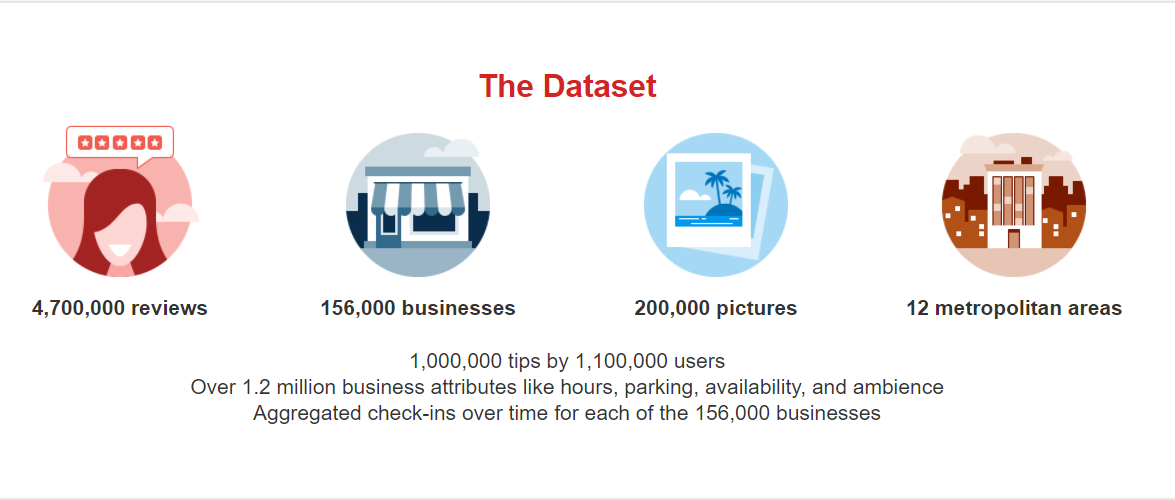
\includegraphics[scale=0.5]{data_details.png}
				\caption{Dataset Details}
		\end{figure}
		\subsection{Analysis}
		We did an initial analysis of the dataset. Below sections present our analysis.
			\subsubsection{User data}
			There are 1,183,362 total users whose reviews are present in the dataset. We plotted a histogram to understand the distribution of user reviews. Looking at the histogram, we can observe that most of the user have very few reviews and some top users have significant number of reviews. Majority of user have 25 or less reviews which is also shown by a mean of 23..72 and standard deviation of 80.5. The maximum number of reviews given by any user is 11656.
			\begin{figure} [H]
				\centering
				\begin{minipage}{.5\textwidth}
					\centering
				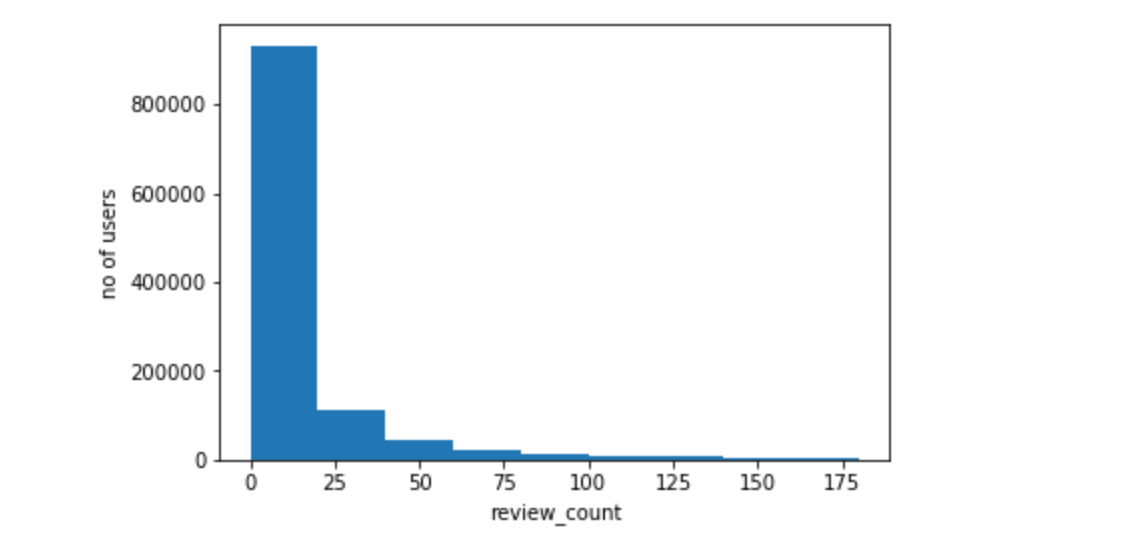
\includegraphics[scale=0.5]{h_user_review.png}
				\caption{Review count per user}
					\label{fig:user_review}
				\end{minipage}%
				\begin{minipage}{.5\textwidth}
					\centering
					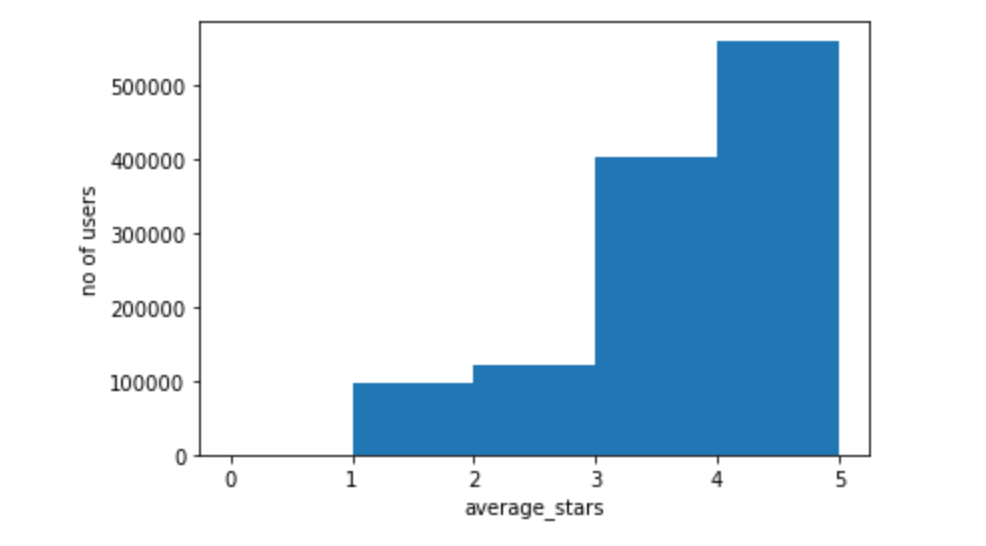
\includegraphics[scale=0.5] {h_user_rating.png}
					\caption{Rating per user}
					\label{fig:user_rating}
				\end{minipage}
			\end{figure}
			
			
		  In addition to number of reviews, we also looked at distribution of star ratings given by a user. Looking at the histogram, we can observe that more users give higher rating which is shown by a median of 3.89 star rating. Mean and standard deviation for the same are 3.71 and 1.10 respectively. In order to group the reviews as positive, average and negative reviews, we have used the following method. We assume that if the rating lies in the range of (mean – standard deviation, mean) which is 2.6 to 3.7, we will categorize it as average. Reviews lower than 2.6 will be considered as a negative review and anything greater than 3.7 will be considered as positive reviews with two extremes being 0 and 1. 
		 
	     We also did some analysis to see the user growth on yelp. User growth has started declining after an increase in users joining from 2005 to 2014 .
	     
	      \begin{figure}[H]
	     	\centering
	     	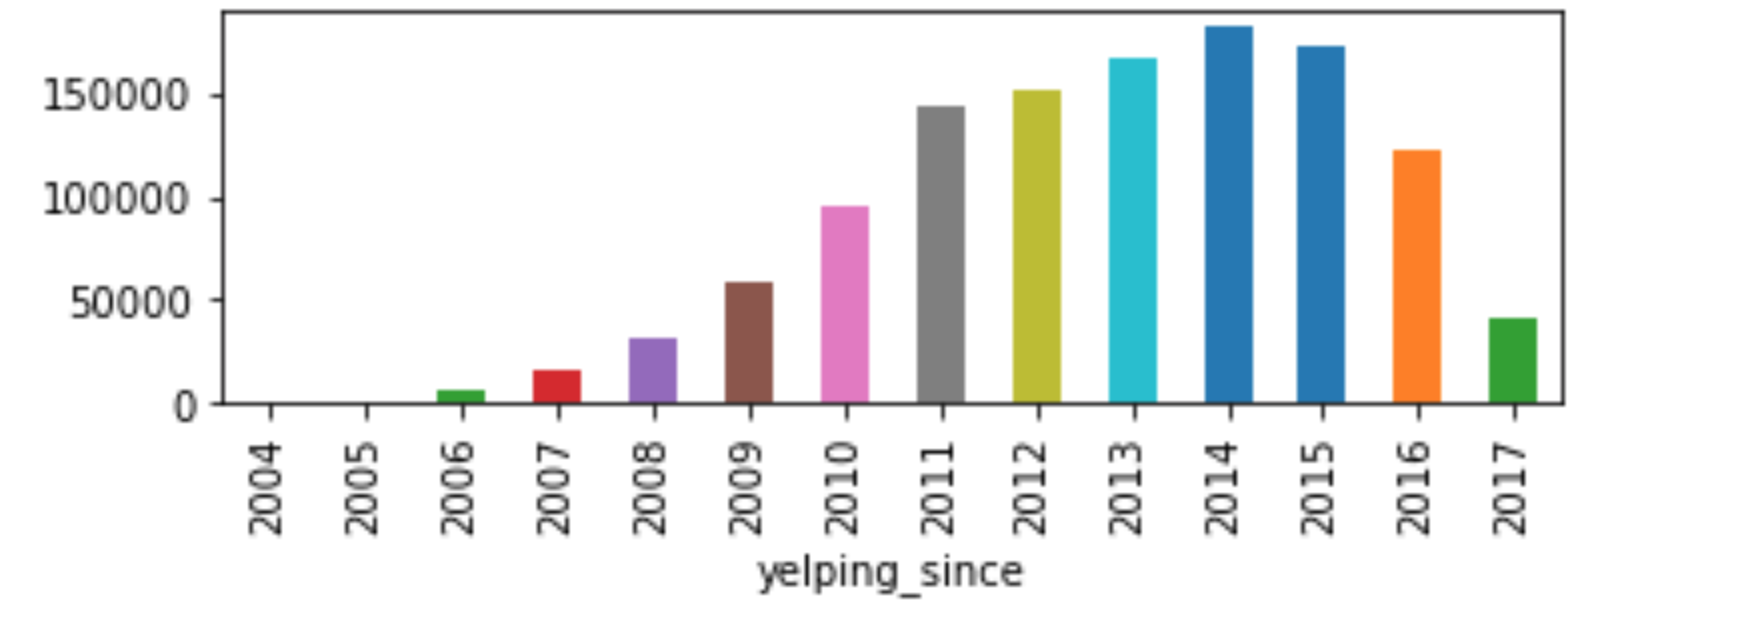
\includegraphics[scale=0.4] {user_growth.png}
	     	\caption{User Growth}
	     \end{figure}
     
     	\subsubsection{Business Data}
     	There are total 1,56,639 business in the dataset. We grouped business according to city and business category to determine popular cities and categories. Below pie-charts give idea about popular cities and categories.

      	\begin{figure}[H]
      		\centering
      		\begin{minipage}{.5\textwidth}
      			\centering
      			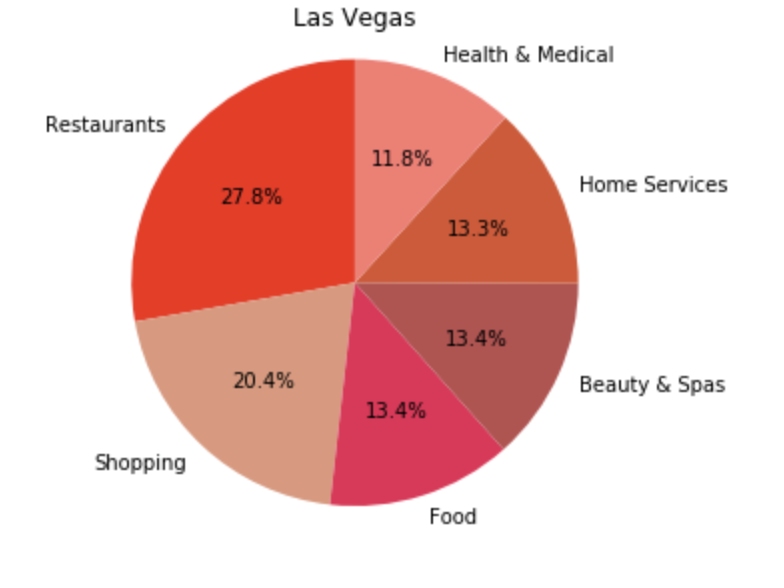
\includegraphics[scale=0.6] {top_cities.png}
      			\caption{Top cities}
      			\label{fig:topcity}
      		\end{minipage}%
      		\begin{minipage}{.5\textwidth}
      			\centering
      		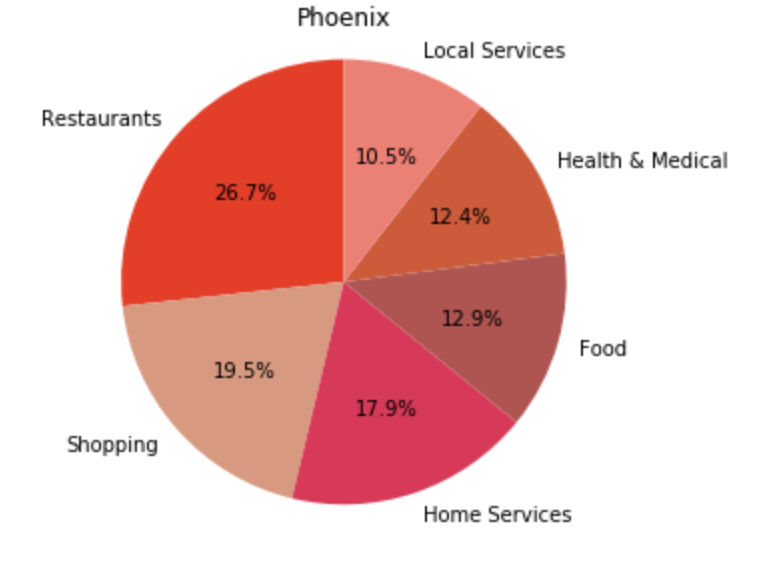
\includegraphics[scale=0.6] {top_categroies.png}
      		\caption{Top Business Categories}
      			\label{fig:topbus}
      		\end{minipage}
      	\end{figure}
      	
 	
	\section{Methods}
		
		\subsection{Clustering Based Approach}
		We use clustering to group users who have similar preferences. For clustering based approach, our inputs are user id, type of business and location of the user. The output of our system is top 20 recommendations of businesses for the above type of business. 
		
		Thus in order to build this recommendation system, we initially divide our training and testing data based on location. So, we only consider users and business from the given location. Our training data consists of user ratings for businesses from 2004 till 2015. Our testing data consists of user ratings for years 2016 and 2017.
		
		We first get the preference of each user by using top 15 categories for the above type of business in the location provided in input. So assuming we have type of business as Restaurants, then top 15 categories could be Indian, American, Bar and Grill, Chinese, so on and so forth. We denote this in form of a vector with elements in it where each element corresponds to each of the top 15 categories. Then for each of those categories, we get all the reviews the user has given for it. We average out the review value and assign the output as a value for that category. If the user has not reviewed a particular category we give the category a value of 3.15 which is the average pf 2.6 and 3.7. 2.6 and 3.7 is the range of our average review as mentioned in the pre-processing part. Thus we create a user preference vector with 15 values.
		
		Next, we create a business vector. This is because in order to recommend a business to a user, we need to create a similar preference vector as above for each business. We have the categories for which each business belongs to. Thus, we have a list of categories for each business. If at least 3 of the top categories are part of a business, then that business can be recommended to a user. After filtering out valid business which we can recommend, we create a business vector exactly like the user's preference vector. It is important to know that index of any category in user preference vector should correspond to index of that category in business vector. Also we take care that if a particular category is not reviewed in a particular business, then thst business does not serve thst category. So we assign a score of 1 to those categories in business vector.
		
		After this, we use Agglomerative Hierarchical Clustering\cite{agg} to cluster users. This method builds the hierarchy from the individual elements by progressively merging clusters using a distance metric. In our case we use Minkowski distance which is given by :
		
		\[
		\left(\sum_{i=1}^{n} \left | x_i - y_i \right |^p  \right )^\frac{1}{p}
		\]
		
		Thus we can calculate distance between user preference vectors using the formula above where n = 15. After calculating distances between every pair of user preference vector, we merge the two clusters with minimum distance and iteratively continue until we are left with only cluster. However if everything is in one cluster, then clustering does not help us that much. Thus we continue merging until we are left with 15 clusters where 15 denotes the number of categories we are using to create the preference vector. A sample dendogram after performing Clustering for Restaurants in the city of Stuttgart is given below: 
		
		 \begin{figure}[H]
	     	\centering
	     	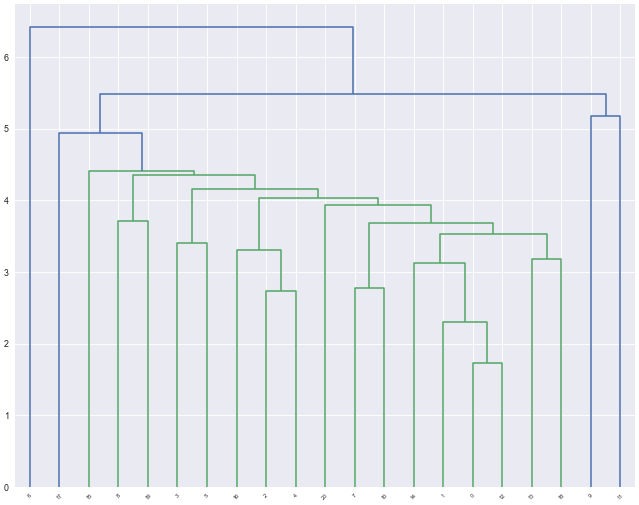
\includegraphics[scale=0.3] {clust.png}
	     	\caption{Dendogram of Clustering for Restaurants in the city of Stuttgart}
	     \end{figure}

		
		X-Values of the dendogram represents the indexes of users and the y-axis of dendogram represents the measure of closeness between each user. After clustering, using the index we can determine which cluster our target user belongs to. Then we average out the preference vector for all users in the cluster and get an average preference vector. We then take dot product between the output average preference vector and each business vector to get similarity. Thus if the dot product is 0 that means the two vectors are 90 degrees apart and dissimilar. However, as the dot product increases, the two vectors converge and come close to each other. So, the business vector with which we get the highest dot product will be recommended first in our recommendation system.
				
		\subsection{Collaborative Filtering}
		Collaborative filtering(CF) is a method of making automatic predictions (filtering) about the interests of a user by collecting preferences or taste information from many users (collaborating). For the purpose of this project we evaluate two strategies for CF:
		\begin{itemize}
			\item{user - user based recommendations}
		\end{itemize}

		We create a n X m matrix, where n is the number of users and m is the number of business, with each cell representing the rating given by a user to that particular business. Each row in matrix represent the vector of star rating given by user for all the businesses.
		
		While doing this, we face two issues and resolved them as mentioned 1. As expected, there are lot of missing values in matrix(for business which user has not given rating). We treat missing values as the average computed after following the second step - which will always be zero.
2. There is an issue of handling the rating given by soft users and hard users i.e some users may rate the business they like with a 3 star ratings and there are some users who may rate the business they don't like with a 3 star ratings. To normalize these ratings for each user we use the centered cosine similarity. We normalize the ratings by subtracting the row mean for each user.\cite{vid1}

		For predicting the rating for the new business by user, we modified the functions given in HW3 of coursework. We used the similarity matrix to found top 10 similar users who have given rating to that items. Then we computed the weighted average of ratings based on similarity between the target user and other users.
		
		$$Prediction_t = \frac{\sum_{u=1}^{10} mat[u][i] * sim_{ut}} {\sum_{u=1}^{10}}$$ 
		
	 $$Prediction Rating for User t $$
	
		
		Finally for recommending the Top 10 business to user, we computes the prediction rating of all the business which user has not rated, based on similar users. Then we recommend the top 10 business with maximum prediction of rating value. \\
		\begin{itemize}
			\item{Matrix Factorization}
		\end{itemize} 
		
	 
	
	 

		
		To recommend new businesses to a target user 'target', we find the cosine similarity between all other users and 'target'. Top 'k' businesses rated with positive average star rating, by users of having cosine similarity greater than 1, will be recommended to user 'target'.\cite{vid2}
	
		\subsection{Deep Learning Method} 
		We have using Neural Collaborative Filtering \cite{ncf} (NCF) approach suggested by Xiangnan He and team. We looked at various deep learning approaches towards building recommendation systems and choose this work as it was generally applicable compared to other techniques which either target music or video recommendations specifically. NCF uses multi-layers perceptron to learn use-item interaction function. It is generic and tries to generalize matrix factorization under its framework. This work focuses on the implicit feedback which indirectly reflects users behaviors.
		
		\subsubsection{Notation and Problem Formulation} 
		Let M and N denote the number of users and items, respectively. User-item interaction matrix $Y \in \mathbb{R}^{M \times N}$ from user's implicit feedback is defined as,
		\[
			y_{ui} = \begin{Bmatrix}
			1, & \text{if interaction (user u, item i) is observed} \\
			0, & otherwise
			\end{Bmatrix}
		\] 
		The recommendation problem with implicit feedback is
		formulated as the problem of estimating the scores of unobserved
		entries in Y, which are used for ranking the items.
		
		\subsubsection{Neural Collaborative Filtering}
		A multi-layer representation is used to model user-item interaction $y_{ui}$ as shown in below figure.
		\begin{figure}[H]
			\label{fig:ncf}
			\centering
			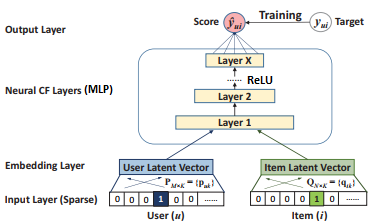
\includegraphics[scale=1.2]{ncf.png}
			\caption{Neural Collaborative Filtering Model}
		\end{figure}
		The bottom input layer consists of two feature vectors $v_{u}^{U}$ and $v_{i}^{I}$ that describe user u and item i, respectively. As it is purely collaborative model, only user and item ids are taken as input in form of one-hot vectors. Above the input layer is the embedding layer; it is a fully connected layer that projects the sparse representation to a dense vector. The user embedding and item embedding are then fed into a multi-layer perceptron architecture to map the latent vectors to prediction scores.  The final output layer is the predicted score $\hat{y_{ui}}$, and training is performed by minimizing the point-wise loss between $\hat{y_{ui}}$
		and its target value $y_{ui}$
		
	\section{Experiments and Results}
	\subsection{Data Pre-processing}
	Initially, we filtered business by only considering restaurants category to reduce noise in our model. In addition, we removed users who had less than 20 reviews for restaurant type business so that we have enough information about users and to also reduce sparsity of data. We also created 99 negative samples for each selected user for evaluation of deep learning approach. We kept the latest review of the selected user as the test data. Overall, after pre-processing, we had 19,771 users, 48,349 businesses , 90,8436 reviews for training and 19,771 reviews for testing.
	
	
	\subsection{Clustering Based Approach}
	\subsubsection{Calculating Similarity and Generating Recommendations}
	Based on recommendations received from our cluster, we use two measures to analyze our recommendation system namely Hit-Ratio (HR) and Normalized discounted cumulative gain (NDCG). If our user visits any of the recommended business in our testing data, we check what rating has he given to that business. If the rating falls in the positive review range as mentioned in the pre-processing part, then we increment the hit score by 1. If the rating falls in the negative range, we decrement the score by 1. If the rating is in average range then it does not matter as it can be positive or negative. Thus using the above metric we calculate the Hit ratio which is given by: 
	
	\[
	\frac {\sum_{i=1}^{n} Hit Score}{count}
	\]
	Now this hit ratio is calculated for one particular user. We average out the hit score for all the users in the test set. Thus we get an average hit score for recommendations for all the users.
	
In NDCG, we first calculate gain for each recommendation. The gain refers to the actual rating user gives to each business. Cumulative gain refers to summation of each gain for each recommendation. After that we discount each gain by assigning a weight to it. Thus if the recommendation is at the top of list, the gain for that recommendation will have more weight than if the recommendation was at the bottom of the list. Thus our Discounted cumulative gain is calculated based on the formula given below:

	\[
	DCG = \sum_{i=1}^{n}\frac { Review Rating}{i}
	\]
	
	In this case 'i' refers to the index of recommendation. In our case we are recommending top 20 business so 'i' will range from 1 to 20 inclusive. After calculating Discounted Cumulative Gain (DCG) we calculate Ideal Discounted Cumulative Gain (IDCG) which refers to for every recommendation we give a rating of 5. Thus our NDCG becomes:
	
	\[
	NDCG = \frac {DCG}{IDCG}
	\]
	
	After calculating NDCG for one user, we calculate NDCG for every user in the test and average it out.
	
	Below is a table showing calculation of Hit Ratio and NDCG for top 15 cities mentioned in pre-processing. 
	
		
		\begin{table}[htb]

\begin{tabular}{|l|l|l|}
\hline
City        & Hit Ratio & NDCG \\
\hline
Las Vegas   & 0.58      & 0.78 \\
Toronto     & 0.61      & 0.75 \\
Phoenix     & 0.62      & 0.80 \\
Charlotte   & 0.55      & 0.77 \\
Edinburgh   & 0.60       & 0.81  \\
Pittsburgh  & 0.44      & 0.78 \\
Montr�al    & 0.57      & 0.80 \\
Scottsdale  & 0.69      & 0.91 \\
Cleveland   & 0.64      & 0.89 \\
Madison     & 0.64      & 0.78 \\
Stuttgart   & 0.5       & 0.71 \\
Mesa        & 0.41       & 0.52 \\
Tempe       & 0.35      & 0.69 \\
Henderson   & 0.65      & 0.88 \\
Mississauga & 0.22      & 0.63 \\
Average     & 0.55      & 0.78 \\
\hline
\end{tabular}
\centering
\caption{Evaluation Metrics: Hit Ratio and NDCG of top 15 Cities for Restaurants}
\label{res-clustering}
\end{table}


	
	 
	\subsection{User-User Collaborative Filtering}

	For the initial setup, we have worked on 100,000 rows of reviews.json file. We have created a matrix of 78276 users and 4224 businesses.We randomly choose one user to find the set of similar users of count 200. Based on positive average star ratings given by 200 users, 531 set of businesses are recommended to users.
	
	\subsection{Deep Learning Method}
	We used the model implementation \cite{ncfi} provided by original authors to build the model on our dataset. For each training example, first we form one-hot vector for both user and business. Then, we feed these to the embedding layer and concatenate these two to form a single vector. Then, we used four hidden fully connected layers with respectively 64,32,16 and 8 factors and relu activation functions. Finally, we had a fully connected output layer with sigmoid activation function. 
	
	In order to evaluate the trained model, as explained above Hit ratio and NDCG were used. We used 20 epochs to train the model in batch sizes of 256. Results for best model is shown in below table.
	
	\begin{table}[H]
		\begin{tabular}{|c|c|}
		\hline
		Hit Ratio & NDCG \\
		\hline
		0.8197 & 0.6220 \\
		\hline
		\end{tabular}
	\centering
	\caption{Deep learning evaluation: Hit Ratio and NDCG for Restaurants}
	\label{res-dll}
	\end{table}
	
	
	\begin{thebibliography}{99}
		% NOTE: change the "9" above to "99" if you have MORE THAN 10 references.
		
	\bibitem{yelp} Yelp Dataset Challenge \url{https://www.yelp.com/dataset_challenge}
	\bibitem{rsw} Recommendation System Wiki \url{https://en.wikipedia.org/wiki/Recommender_system}
	\bibitem{cfilter}Collaborative filtering \url{https://en.wikipedia.org/wiki/Collaborative_filtering}
		\bibitem{cfiltervid}Collaborative filtering Techniques \url{https://www.youtube.com/watch?v=h9gpufJFF-0}
		\bibitem{mov}Movie Recommenation System \url{https://beckernick.github.io/matrix-factorization-recommender/}
	\bibitem{ydeep} Paul Covington, Jay Adams, Emre Sargin \textit{Deep Neural Networks for YouTube Recommendations}, ACM 2016.
	\bibitem{ncf} Xiangnan He, Lizi Liao, Hanwang Zhang, Liqiang Nie, Xia Hu and Tat-Seng Chua\textit{Neural Collaborative Filtering}, ACM 2017
	\bibitem{vid1} Lecture on CF - Stanford \url{https://www.youtube.com/watch?v=h9gpufJFF-0&t=854s}
	\bibitem{vid2} Recommendation System Netflix \url{https://www.youtube.com/watch?v=bLhq63ygoU8&t=5598s}
	\bibitem{ncfi} NCF Implementation \url{https://github.com/hexiangnan/neural_collaborative_filtering}
	
	\bibitem{agg}Sz�kely, G. J.; Rizzo, M. L. (2005). "Hierarchical clustering via Joint Between-Within Distances: Extending Ward's Minimum Variance Method". Journal of Classification
	
	\end{thebibliography}
	%%%%%%%%%%%%%%%%%%%%%%%%%%%%%%%%%%%%%%%%%
	
	
	
	
	
	
\end{document} 